\section{Résultats et interprétations}

Nous avons fait tourner cette simulation pour une durée totale physique de 26141802 secondes, soit l'équivalent de 302.6 jours. 
Les solutions pour chaque $r$ de la branche supérieure déterminé par dichotomie ne sont pas équivalntes aux branches atteintes dans la simulations. Nous pouvons voir sur la figure (\ref{fig:tau.png}) en rouge la branche déterminer par dichotomie correspondant à $\tau_{ff} = 0.06 $ et en blanc celle correspondant à la valeur théorique $\tau_{ff} = 1$. Les possibles raisons de cet écarts sont dévelopés partie (\ref{sec::pistes}). La simulation est bien en accord avec le passage d'un disque optiquement épais à un disque optiquement mince. Nous pouvons voir figure (\ref{fig:c1.eps}) et (\ref{fig:c20.eps}) comment se comporte le système du point de vue de ces deux grandeurs physiques. \FIXME{parler de l'instabilité} \\


Un des enjeux pour développer cette simulation de disque d'accretion à une dimension autour d'un trou noir serait d'include la singularité à notre système. En effet elle n'intervient que comme condition au bort intéreur pour résoudre les équations sur $T$, $\Sigma$ et $v$. Cela s'avererait cependant d'une complexité bien supérieure puisque nous ne pourions plus considérer le disque en rotation képleienne aux abord du trou noir. Par cet exemple consernant la grandeur physique $v$, nous voyons rapidemment la necessité de prendre en compte des effets relativiste pour comprendre comment la matière est accrété à l'intérieur du trou noir. Bien que les trous noirs soient les objets les plus simple de l'Univers d'un point de vue des paramètres qui le caractérises, la physique de son environnement n'en reste pas moins complexe. 
 

\begin{figure}
  \begin{center}
    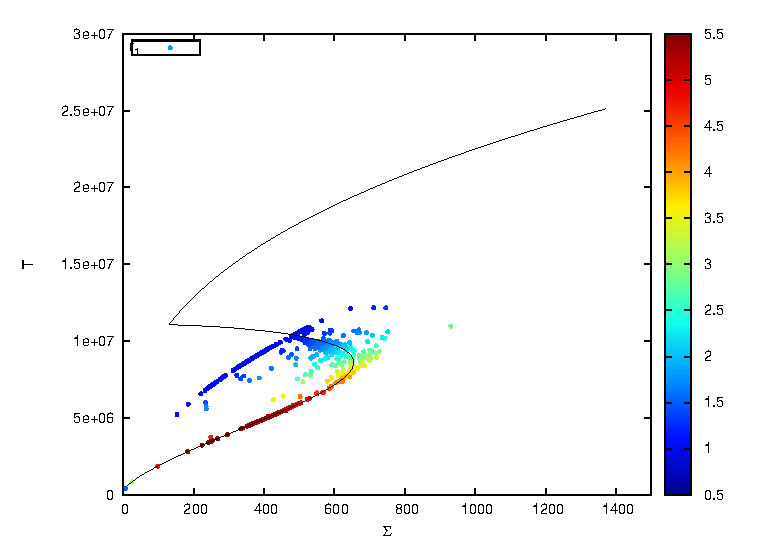
\includegraphics[]{c1.eps}
  \end{center}
  \caption{$T=f(\Sigma)$, $\Delta t = 26141802 s$ (durée de la simulation) pour $r_{1}$. Le gradiant de couleur représente les valeurs de $\tau_{ff}$}
  \label{fig:c1.eps}
\end{figure} 

\begin{figure}
  \begin{center}
    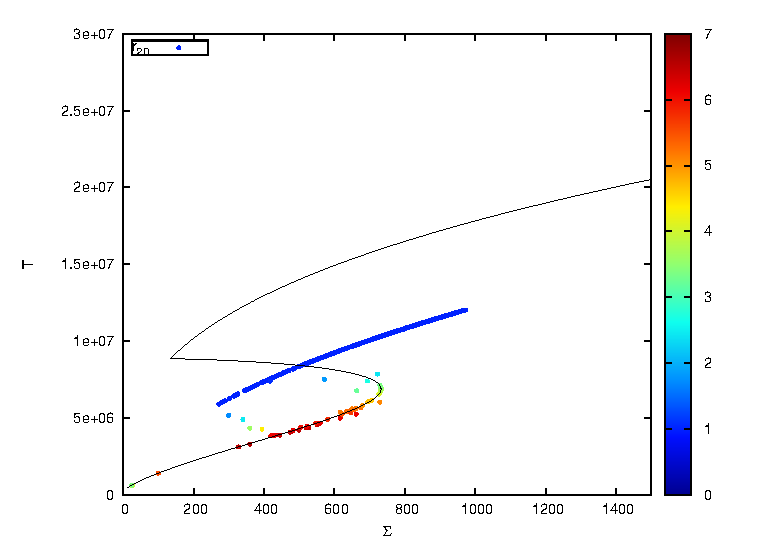
\includegraphics[]{c20.eps}
  \end{center}
  \caption{$T=f(\Sigma)$, $\Delta t = 26141802 s$ (durée de la simulation) pour $r_{20}$. Le gradiant de couleur représente les valeurs de $\tau_{ff}$}
  \label{fig:c20.eps}
\end{figure}


\begin{figure}
  \begin{center}
    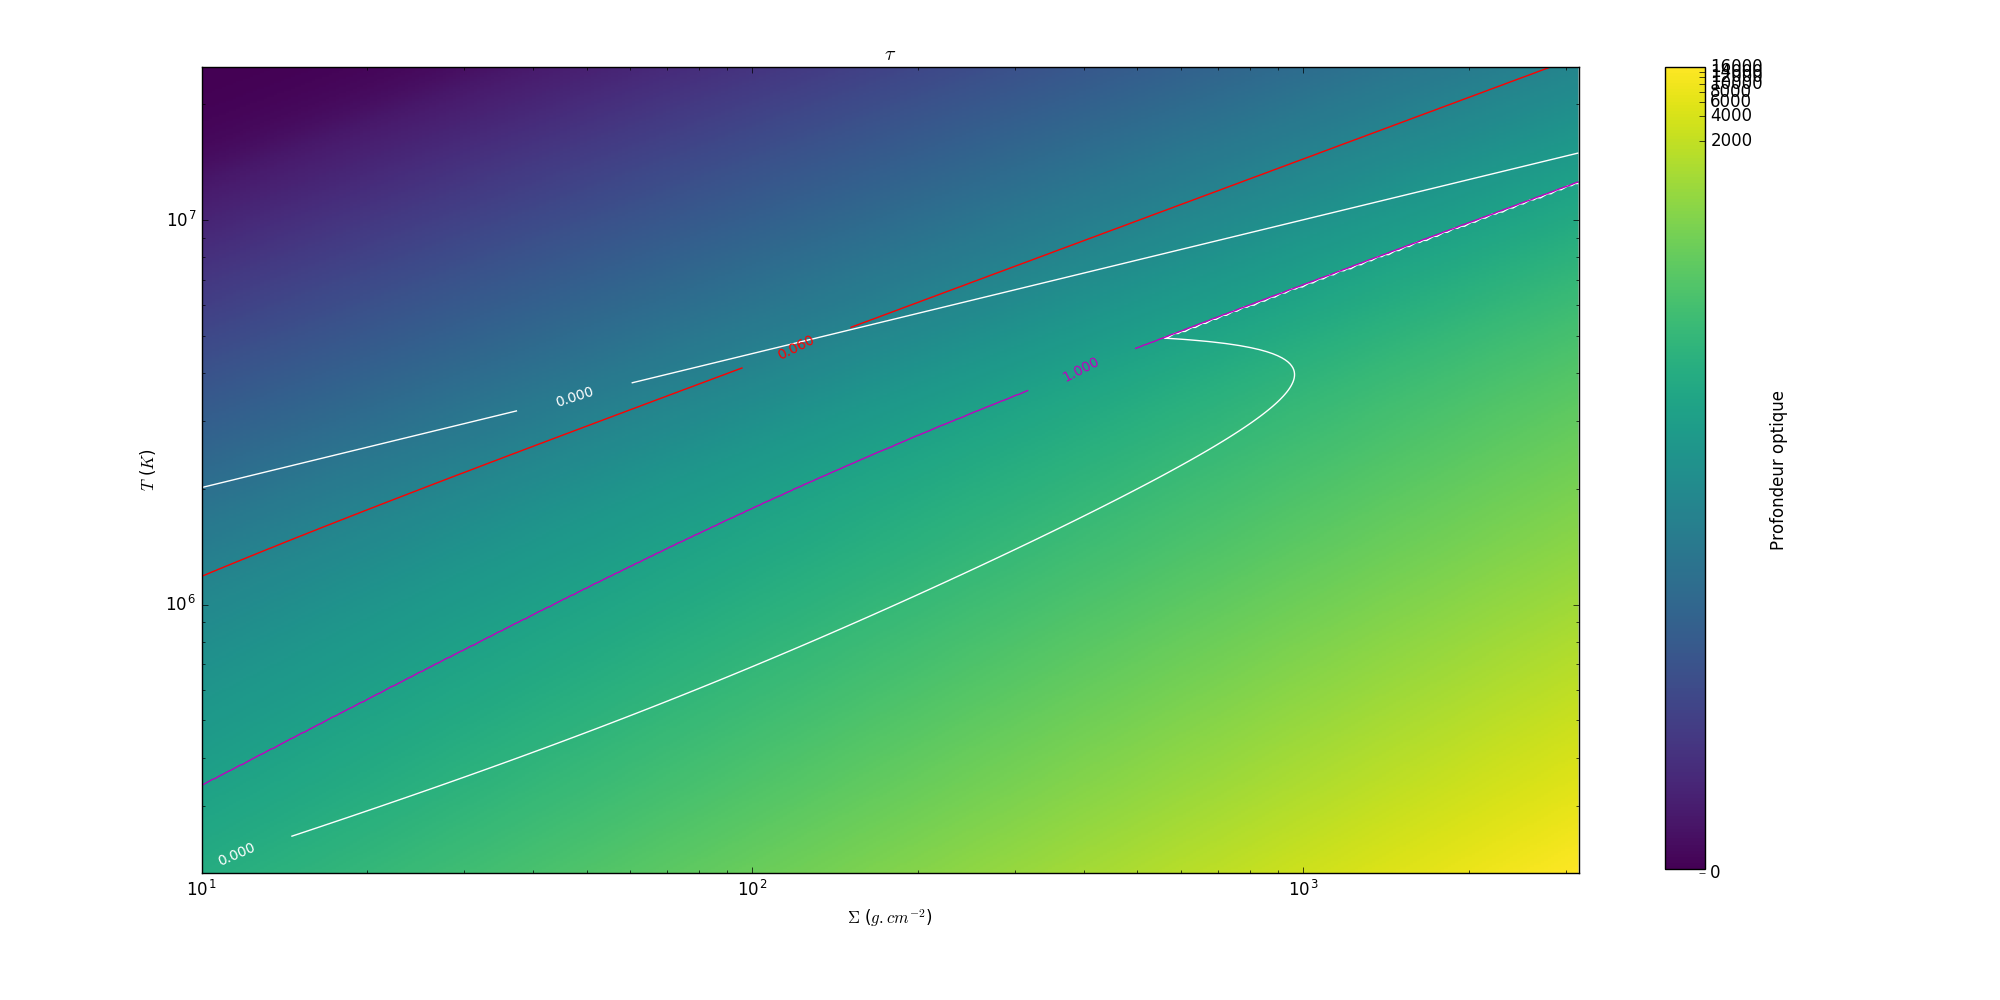
\includegraphics[scale=0.36]{tau.png}
  \end{center}
  \caption{\FIXME{include dans courbe en s peut etre ?}}
  \label{fig:tau.png}
\end{figure} 

